\section{Method}
%======================================================================================

The entire system was created and simulated in Matlab R2023b, Simulink and Stateflow using the model and maze provided by the assignment.

%======================================================================================

\subsection{Differential drive model}
% Detail how you expanded the unicycle model to include the differential drive robot model.

The model provided was expanded to work based on a differential drive model. This was achieved by letting the inputs remain as linear velocity $v$ and angular velocity $\omega$. However the method used to obtain $\dot{x}$, $\dot{y}$ and $\dot{\theta}$ was no longer\:\eqref{eq:unicycle_model}. Instead\:\eqref{eq:left_uni_differential} and\:\eqref{eq:right_uni_differential} was used in combination with\:\eqref{eq:differential_drive_model}. With this, the input and output remained the same, resulting in modeling the system as a whole as a unicycle model, but with the internal workings of a differential drive model.

%======================================================================================

\subsection{Parameters}
% Detail parameters

The system parameters were:
\begin{itemize}
    \item Wheel radius: $r = 0.1$
    \item Wheel base: $l = 0.5$
    \item Follow wall behavior threshold: $\Delta_1 = 1$
    \item Avoid obstacle behavior threshold: $\Delta_2 = 0.5$
    \item Constant velocity: $v = 0.1$
    \item Proportional gain: $P = 10$
    \item Tolerance distance to goal: $\epsilon = 0.01$
    \item Simulation time: $t_s = 1100$
\end{itemize}
Note that parameters included in the model provided are not covered, this includes e.g. start and goal position.
As can be seen from the parameters, only a simple proportional controller was used for control, no $I$ or $D$ part.
All parameters was specified in a initialization Matlab script.

%======================================================================================

\subsection{Designing Behaviors}
% Discuss how you designed the required behaviors:

The different behaviors of the system are detailed in this section, go to goal (GTG), avoid obstacle (AO), follow wall (FW) clockwise (c) and counter clockwise (cc).
A complete version of the go to goal behavior was already present in the provided model, the only development made to this consisted of the transitions from this behavior to others. See Fig.\:\eqref{fig:behavior_transitions} for all transitions between behaviors. The transitions was implemented in Stateflow.
\begin{figure}
    \centering
    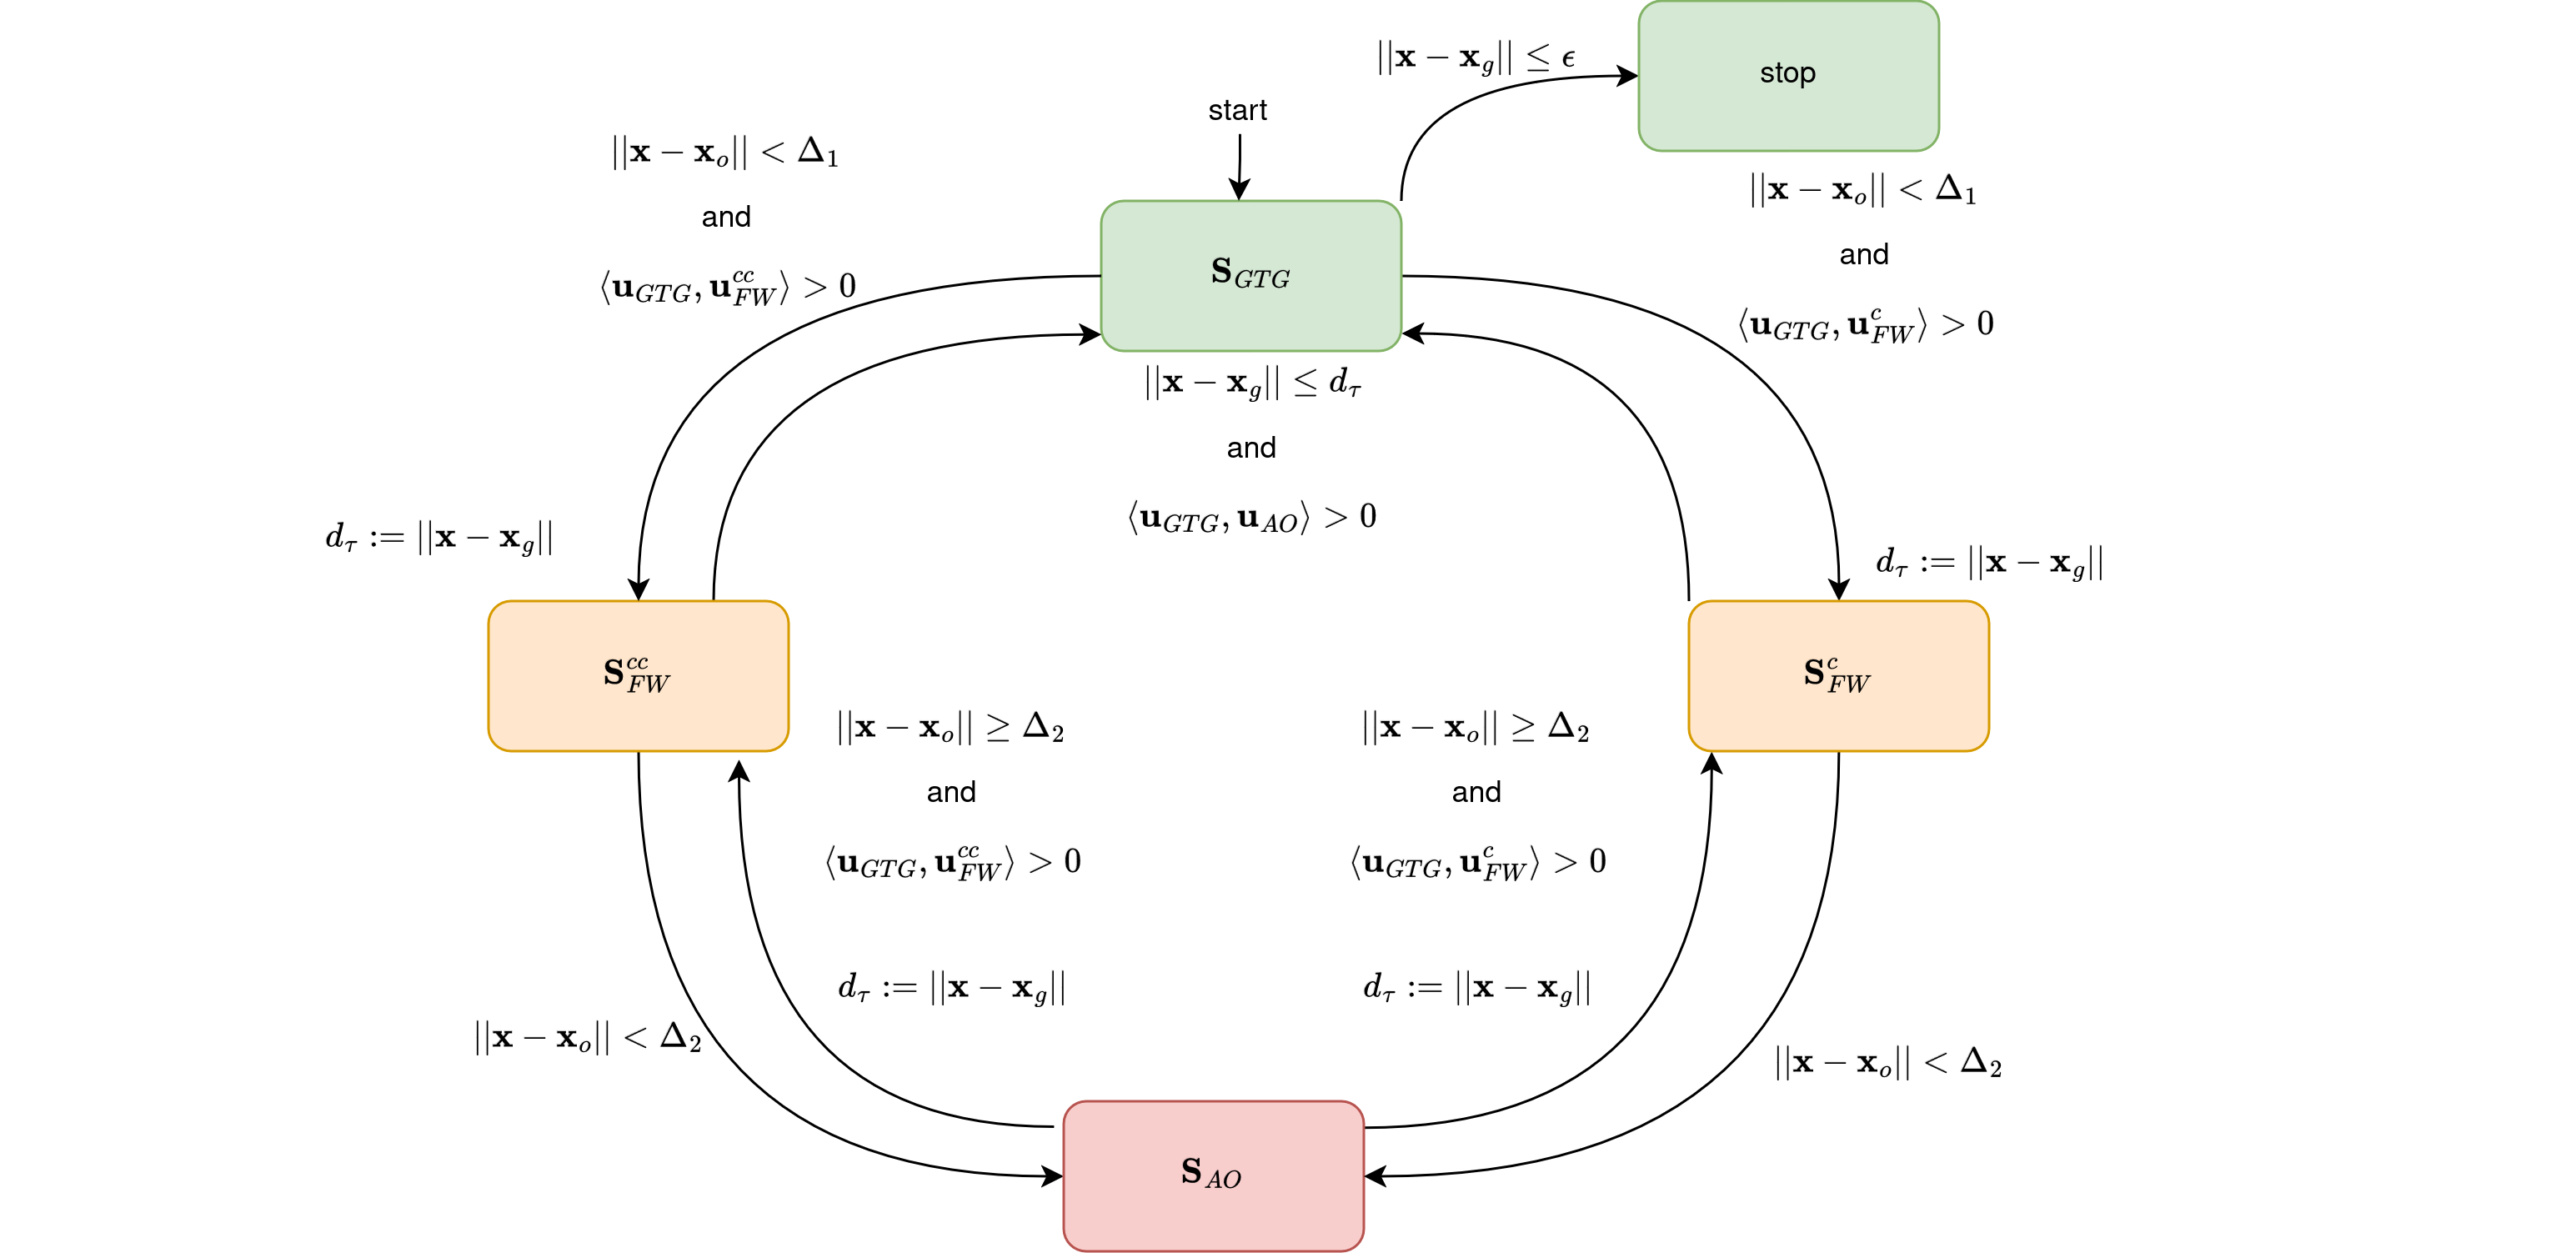
\includegraphics[width=\columnwidth]{images/flowchat_lab1.png}
    \caption{All possible transitions between every behavior.}
    \label{fig:behavior_transitions}
\end{figure}




\subsubsection{Calculations}
All distances were calculated using Euclidean distance, see\:\eqref{eq:euclidean_distance} for 2-D vectors in Euclidean xy-plane, the formula can be further expanded to include vectors of any dimension.
\begin{equation}
    \label{eq:euclidean_distance}
    d = \norm{ \mathbf{x} - \mathbf{x}_p } = \sqrt{(x-x_p)^2 + (y-y_p)^2}
\end{equation}
where $\mathbf{x} = [x,y]^T$ is the robots position and $\mathbf{x}_p = [x_p, y_p]^T$ is an arbitrary target point.
Note that $\mathbf{x}$ refers to a vector (specifically the position vector of the robot), while $x$ refers to a scalar, the x coordinate in Euclidean space.

$d_\tau$ is the distance from the robot to the goal at time $t = \tau$, see\:\eqref{eq:d_tau}.
\begin{equation}
    \label{eq:d_tau}
    d_\tau := \norm{ \mathbf{x}(\tau) - \mathbf{x}_g } = \sqrt{(x(\tau)-x_g)^2 + (y(\tau)-y_g)^2}
\end{equation}
where the subscript $g$ refers to goal.

$\langle *, * \rangle$ refers to the dot product between two vectors, sometime also written as $*\cdot*$. The dot product describes if the angle between two vectors is less than $\frac{\pi}{2}$ ($\langle *, * \rangle > 0$), equal to $\frac{\pi}{2}$ ($\langle *, * \rangle = 0$), or more than $\frac{\pi}{2}$ ($\langle *, * \rangle < 0$). Three different dot products are necessary for this system, see\:\eqref{eq:angle_goal_ao},\:\eqref{eq:angle_goal_c} and\:\eqref{eq:angle_goal_cc}\:\cite{carlenerikssonLectureKinematicsBehavioral2024}. 
\begin{dmath}
    \label{eq:angle_goal_ao}
    \langle \mathbf{u}_{GTG} , \mathbf{u}_{AO} \rangle
\end{dmath}
\begin{dmath}
    \label{eq:angle_goal_c}
    \langle \mathbf{u}_{GTG} , \mathbf{u}_{FW}^{c} \rangle
\end{dmath}
\begin{dmath}
    \label{eq:angle_goal_cc}
    \langle \mathbf{u}_{GTG} , \mathbf{u}_{FW}^{cc} \rangle
\end{dmath}
(Note that standard dot product in Euclidean space is commutative.)
Where $\mathbf{u}_{GTG}$, $\mathbf{u}_{AO}$, $\mathbf{u}_{FW}^{c}$ and $\mathbf{u}_{FW}^{cc}$ can be obtained according to\:\eqref{eq:u_gtg},\:\eqref{eq:u_ao},\:\eqref{eq:u_fw_c} and\:\eqref{eq:u_fw_cc}\:\cite{carlenerikssonLectureKinematicsBehavioral2024}.
\begin{dmath}
    \label{eq:u_gtg}
    \mathbf{u}_{GTG} = \mathbf{x}_g - \mathbf{x}
\end{dmath}
\begin{dmath}
    \label{eq:u_ao}
    \mathbf{u}_{AO} = \mathbf{x} - \mathbf{x}_o
\end{dmath}
\begin{dmath}
    \label{eq:u_fw_c}
    \mathbf{u}_{FW}^{c} = \mathbf{R}_{\text{z}}(-\pi/2) \mathbf{u}_{AO}
\end{dmath}
\begin{dmath}
    \label{eq:u_fw_cc}
    \mathbf{u}_{FW}^{cc} = \mathbf{R}_{\text{z}}(\pi/2) \mathbf{u}_{AO}
\end{dmath}
Note that in this specific case where all the vectors are in the 2-D Euclidean xy-plane, and thus of dimension 2, then $\mathbf{R}_{\text{z}}(\phi) \in \mathbb{R}^{2\times2}$ (note that the $\text{z}$ could be omitted but is included for clarity).

All the angles in the system were constrained to the interval $[-\pi, \pi]$ using the $\atantwo(y,x)$ function.




\subsubsection{Transitions}
There are multiple transitions between each behavior, all described in Fig.\:\ref{fig:behavior_transitions}. The transitions will also be described here for additional clarity. The transitions will be presented in terms of equations, if all the equation conditions hold, then the transition is executed.

% GTG
Go to goal had three possible transitions: stop simulation (goal reached), follow wall clockwise and follow wall counter clockwise.
Transition from go to goal to stop simulation was executed if\:\eqref{eq:gtg_to_ss} was satisfied.
\begin{equation}
    \label{eq:gtg_to_ss}
    \norm{ \mathbf{x} - \mathbf{x}_g } \le \epsilon
\end{equation}
Transition from go to goal to follow wall clockwise was executed if\:\eqref{eq:gtg_to_fw_c} was satisfied. At the particular time instant $\tau$ at which this transition was executed, $d_{\tau}$\:\eqref{eq:d_tau} was saved.
\begin{equation}
    \label{eq:gtg_to_fw_c}
    \begin{cases}
         \norm{ \mathbf{x} - \mathbf{x}_o } < \Delta_1 \\
         \langle \mathbf{u}_{GTG} , \mathbf{u}_{FW}^{c} \rangle > 0
    \end{cases}
\end{equation}
Transition from go to goal to follow wall counter clockwise was executed if\:\eqref{eq:gtg_to_fw_cc} was satisfied. At the particular time instant $\tau$ at which this transition was executed, $d_{\tau}$\:\eqref{eq:d_tau} was saved.
\begin{equation}
    \label{eq:gtg_to_fw_cc}
    \begin{cases}
         \norm{ \mathbf{x} - \mathbf{x}_o } < \Delta_1 \\
         \langle \mathbf{u}_{GTG} , \mathbf{u}_{FW}^{cc} \rangle > 0
    \end{cases}
\end{equation}

% FW C
Follow wall clockwise had two possible transitions: go to goal and avoid obstacles.
Transition from follow wall clockwise to go to goal was executed if\:\eqref{eq:fw_c_to_gtg} was satisfied.
\begin{equation}
    \label{eq:fw_c_to_gtg}
    \begin{cases}
        \norm{ \mathbf{x} - \mathbf{x}_g } \le d_{\tau} \\
        \langle \mathbf{u}_{GTG} , \mathbf{u}_{AO} \rangle > 0
    \end{cases}
\end{equation}
Transition from follow wall clockwise to avoid obstacle was executed if\:\eqref{eq:fw_c_to_ao} was satisfied.
\begin{equation}
    \label{eq:fw_c_to_ao}
    \begin{cases}
        \norm{ \mathbf{x} - \mathbf{x}_o } < \Delta_2
    \end{cases}
\end{equation}

% FW CC
Follow wall counter clockwise had two possible transitions: go to goal and avoid obstacles. Note that these transition conditions are identical to the previous two for follow wall clockwise.
Transition from follow wall counter clockwise to go to goal was executed if\:\eqref{eq:fw_cc_to_gtg} was satisfied.
\begin{equation}
    \label{eq:fw_cc_to_gtg}
    \begin{cases}
        \norm{ \mathbf{x} - \mathbf{x}_g } \le d_{\tau} \\
        \langle \mathbf{u}_{GTG} , \mathbf{u}_{AO} \rangle > 0
    \end{cases}
\end{equation}
Transition from follow wall counter clockwise to avoid obstacle was executed if\:\eqref{eq:fw_cc_to_ao} was satisfied.
\begin{equation}
    \label{eq:fw_cc_to_ao}
    \begin{cases}
        \norm{ \mathbf{x} - \mathbf{x}_o } < \Delta_2
    \end{cases}
\end{equation}

% AO
Avoid obstacles had two possible transitions: follow wall clockwise and follow wall counter clockwise.
Transition from avoid obstacles to follow wall clockwise was executed if\:\eqref{eq:ao_to_fw_c} was satisfied. At the particular time instant $\tau$ at which this transition was executed, $d_{\tau}$\:\eqref{eq:d_tau} was saved.
\begin{equation}
    \label{eq:ao_to_fw_c}
    \begin{cases}
        \norm{ \mathbf{x} - \mathbf{x}_o } \ge \Delta_2 \\
        \langle \mathbf{u}_{GTG} , \mathbf{u}_{FW}^{c} \rangle > 0
    \end{cases}
\end{equation}
Transition from avoid obstacles to follow wall counter clockwise was executed if\:\eqref{eq:ao_to_fw_cc} was satisfied. At the particular time instant $\tau$ at which this transition was executed, $d_{\tau}$\:\eqref{eq:d_tau} was saved.
\begin{equation}
    \label{eq:ao_to_fw_cc}
    \begin{cases}
        \norm{ \mathbf{x} - \mathbf{x}_o } \ge \Delta_2 \\
        \langle \mathbf{u}_{GTG} , \mathbf{u}_{FW}^{cc} \rangle > 0
    \end{cases}
\end{equation}




\subsubsection{Behavior}
The desired angle, $\theta_{ref}$ ($\theta_{desired}$), is dependent on the behavior currently being followed. When go to goal behavior is being followed, then $\theta_{ref}$ is calculated according to\:\eqref{eq:theta_gtg}. 
\begin{equation}
    \label{eq:theta_gtg}
    \theta_{ref} = \theta_{GTG} = \atantwo(y_{GTG}, x_{GTG})
\end{equation}
During avoid obstacle behavior it is calculated according to\:\eqref{eq:theta_ao}. 
\begin{equation}
    \label{eq:theta_ao}
    \theta_{ref} = \theta_{AO} = \atantwo(y_{AO}, x_{AO})
\end{equation}
Lastly, for wall follow clockwise and counter clockwise, it is calculated according to\:\eqref{eq:theta_wf_c} and\:\eqref{eq:theta_wf_cc} respectively.
\begin{equation}
    \label{eq:theta_wf_c}
    \theta_{ref} = \theta_{FW\_c} = \atantwo(y_{FW\_c}, x_{FW\_c})
\end{equation}
\begin{equation}
    \label{eq:theta_wf_cc}
    \theta_{ref} = \theta_{FW\_cc} = \atantwo(y_{FW\_cc}, x_{FW\_cc})
\end{equation}

Where all the $y$ and $x$ are the y and x components of their respective $\mathbf{u}$ vectors, see \eqref{eq:u_gtg}, \eqref{eq:u_ao}, \eqref{eq:u_fw_c}, \eqref{eq:u_fw_cc}.

%======================================================================================


%======================================================================================
\begin{comment}
    
\end{comment}
%======================================================================================